\documentclass[]{article}
\usepackage{lmodern}
\usepackage{amssymb,amsmath}
\usepackage{ifxetex,ifluatex}
\usepackage{fixltx2e} % provides \textsubscript
\ifnum 0\ifxetex 1\fi\ifluatex 1\fi=0 % if pdftex
  \usepackage[T1]{fontenc}
  \usepackage[utf8]{inputenc}
\else % if luatex or xelatex
  \ifxetex
    \usepackage{mathspec}
  \else
    \usepackage{fontspec}
  \fi
  \defaultfontfeatures{Ligatures=TeX,Scale=MatchLowercase}
\fi
% use upquote if available, for straight quotes in verbatim environments
\IfFileExists{upquote.sty}{\usepackage{upquote}}{}
% use microtype if available
\IfFileExists{microtype.sty}{%
\usepackage{microtype}
\UseMicrotypeSet[protrusion]{basicmath} % disable protrusion for tt fontshttps://de.overleaf.com/project/5e85b0680d0bed00011ea790
}{}
\usepackage[margin=1in]{geometry}
\usepackage{hyperref}
\hypersetup{unicode=true,
            pdftitle={The dating of the Human-Neandertal introgression event estimated from present-day human genomes is compatible with a multitude of admixture durations},
            pdfauthor={Leonardo Nicola Martin Iasi (Max Planck Institute for Evolutionary Anthropology, MPI EVA), Dr.~Benjamin Marco Peter (MPI EVA, benjamin\_peter@eva.mpg.de)},
            pdfborder={0 0 0},
            breaklinks=true}
\urlstyle{same}  % don't use monospace font for urls
\usepackage{natbib}
\bibliographystyle{plainnat}
\usepackage{graphicx,grffile}
\makeatletter
\def\maxwidth{\ifdim\Gin@nat@width>\linewidth\linewidth\else\Gin@nat@width\fi}
\def\maxheight{\ifdim\Gin@nat@height>\textheight\textheight\else\Gin@nat@height\fi}
\makeatother
% Scale images if necessary, so that they will not overflow the page
% margins by default, and it is still possible to overwrite the defaults
% using explicit options in \includegraphics[width, height, ...]{}
\setkeys{Gin}{width=\maxwidth,height=\maxheight,keepaspectratio}
\IfFileExists{parskip.sty}{%
\usepackage{parskip}
}{% else
\setlength{\parindent}{0pt}
\setlength{\parskip}{6pt plus 2pt minus 1pt}
}
\setlength{\emergencystretch}{3em}  % prevent overfull lines
\providecommand{\tightlist}{%
  \setlength{\itemsep}{0pt}\setlength{\parskip}{0pt}}
\setcounter{secnumdepth}{0}
% Redefines (sub)paragraphs to behave more like sections
\ifx\paragraph\undefined\else
\let\oldparagraph\paragraph
\renewcommand{\paragraph}[1]{\oldparagraph{#1}\mbox{}}
\fi
\ifx\subparagraph\undefined\else
\let\oldsubparagraph\subparagraph
\renewcommand{\subparagraph}[1]{\oldsubparagraph{#1}\mbox{}}
\fi

%%% Use protect on footnotes to avoid problems with footnotes in titles
\let\rmarkdownfootnote\footnote%
\def\footnote{\protect\rmarkdownfootnote}

%%% Change title format to be more compact
\usepackage{titling}

% Create subtitle command for use in maketitle
\providecommand{\subtitle}[1]{
  \posttitle{
    \begin{center}\large#1\end{center}
    }
}

\setlength{\droptitle}{-2em}

  \title{The dating of the Human-Neandertal introgression event estimated from present-day human genomes is compatible with a multitude of admixture durations}
    \pretitle{\vspace{\droptitle}\centering\huge}
  \posttitle{\par}
    \author{Leonardo Nicola Martin Iasi (Max Planck Institute for Evolutionary
Anthropology, MPI EVA), Benjamin Marco Peter (MPI EVA,
\href{mailto:benjamin_peter@eva.mpg.de}{\nolinkurl{benjamin\_peter@eva.mpg.de}})}
    \preauthor{\centering\large\emph}
  \postauthor{\par}
      \predate{\centering\large\emph}
  \postdate{\par}
    \date{2020-09-30}

\usepackage{setspace}
\doublespacing
\usepackage[none]{hyphenat}
\usepackage{amsfonts}
\usepackage{amssymb}
\usepackage{graphicx}
\usepackage{float}
\usepackage{xcolor}
\floatplacement{figure}{H}

\begin{document}
\maketitle

\section{Abstract}\label{abstract}

\section{Introduction}\label{introduction}



\subsection{(Archaic) Interbreeding, genomic consequences and why is it interesting}\label{(Archaic) Interbreeding, genomic consequences and why is it interesting}

The sequencing of Neandertal \citep{green_draft_2010,prufer_complete_2013,prufer_high-coverage_2017, mafessoni_high_coverage_2020} and Denisovan genomes \citep{reich_genetic_2010, meyer_high-coverage_2012} revealed that modern humans outside of Africa interacted, and admixed with these archaic hominins \citep{vernot_resurrecting_2014,fu_genome_2014,fu_early_2015,sankararaman_genomic_2014,sankararaman_combined_2016,vernot_excavating_2016,malaspinas_genomic_2016}. There are two major lines of evidence: First, Neandertals are genome-wide more similar to non-Africans than to Africans \citep{green_draft_2010, meyer_high-coverage_2012}. This shift can be explained by 2-4\% of admixture from Neandertals into non Africans \citep{green_draft_2010, prufer_complete_2013}. Similarly, East Asians and Papuans are more similar to Denisovans \citep{meyer_high-coverage_2012} than other human groups, which is likely due to gene flow from Denisovans. 

In addition, all non-Africans carry genomic segments that are very similar to the sequenced archaic genomes. As these putative \emph{admixture segments} are up to several hundred kilobases (kb) in length, they are unlikely to predate the split of modern humans from Neandertals and Denisovans. Rather, they entered the modern human populations later through gene flow \citep{sankararaman_date_2012, sankararaman_genomic_2014, sankararaman_combined_2016, vernot_resurrecting_2014, vernot_excavating_2016, skov_detecting_2018, skov_nature_2020}. 

Conceptually, these admixture segments arise through recombination: The offsprings of an archaic and modern human parent will have full chromosomes of either ancestry. If this individual has offspring in a largely modern human population, meiotic recombination progressively breaks the archaic chromosome down into smaller and smaller segments, whose size decrease with time \citep{falush_inference_2003, liang_lengths_2014, gravel_population_2012}. Correspondingly, early modern humans such as the 45,000 year old \textit{Ust'Ishim} individual have much longer admixture segments than present-day people \citep{fu_genome_2014}. Assuming that recombination events are independent from each other, the expected length of these admixture segments is roughly inversely proportional to the number of generations since gene flow happened. Hence, using this ``recombination clock'', the length distribution of introgressed chromosomal segments can be used to infer the time of an
admixture event \citep{moorjani_history_2011,pugach_dating_2011,sankararaman_date_2012,loh_inferring_2013,sankararaman_combined_2016,pugach_gateway_2018,jacobs_multiple_2019,hellenthal_genetic_2014,pool_inference_2009,moorjani_history_2011,gravel_population_2012,liang_lengths_2014}.

Here, we primarily focus on the overlap of Neandertals and modern humans in Eurasia, and the timing of the resulting gene flow. As no Neandertals have been found in Africa, the potential period of contact starts with the Out-Of-Africa event, whereas the latest gene flow would be the disappearance of Neandertals. The earliest modern human remains outside of Africa are directly dated to around 188 thousand years ago (kya)  using a combination of uranium-thorium, uranium-series and electron spin resonance dating techniques  \citep{stringer_when_2018,hershkovitz_earliest_2018} and a possible extinction of Neandertals is suggested to be around 37 kya (radiocarbon and luminescent dating of a Neandertal site in Spain \citep{zilhao_precise_2017}) and 39 kya (radiocarbon dates of Neandertal sites across Europe \citep{higham_timing_2014}). This leaves a potential time frame for Neandertal and modern human interaction of approximately 140,000 years. However, direct evidence of modern humans and Neandertals in the same geographical location at the same time is much spottier; in Europe, for example Neandertals and modern humans likely overlapped only for less than 10,000 years \citep{bard_extended_2020}. Detailed genetic dating of when Neandertals and modern human admixture started and ended could thus make the dating of these events more precise.

\subsection{Admixture models}\label{Admixture models}

 Dates of Admixture events can be estimated by modeling the admixture segment length distribution. The simplest models assume that admixture segments are rare and inbreeding is not significant, such that admixture segments are unlikely to recombine with each other \citep{pool_inference_2009,liang_lengths_2014}. Further assumptions are that the segments act neutrally \citep{shchur_distribution_2019} and the recombination clock is constant over time and populations \citep{gravel_population_2012}. In addition, it is generally assumed that the admixture happens over a very short time period, in a single \textit{admixture pulse} \citep{moorjani_history_2011}, usually modelled as a single generation of interbreeding.


\subsection{The two approaches and their application to find archaic admixture dates}\label{the-two-approaches-and-their-application-to-find-archaic-admixture-dates}
The first step in dating admixture events from genetic data is therefore estimating the length distribution of admixture segments.  There are two main approaches for this; a first sets of methods starts with identifying all admixture segments over a certain length, and then use the length distribution of these segments for inference. Alternatively, the length distribution can also be estimated from patterns of linkage along a chromosome directly, without explicitly inferring the genomic location of these segments (\citep{chimusa_dating_2018}) (Figure \ref{fig:fig1} B).

 In the first set of approaches, the identification of segments is largely independent from the later dating, and can be done using a variety of methods \citep{racimo_signatures_2017,seguin_orlando_paleogenomics_2014,vernot_excavating_2016,sankararaman_combined_2016,skov_detecting_2018}. These approaches are most useful for recent admixture estimated on high-quality data, as uncertainty in the segment identification is not easily fed forward into the timing inference \citep{hellenthal_genetic_2014}.

Thus, methods using admixture-induced linkage disequilibrium (ALD) are more widely used \citep{moorjani_history_2011,sankararaman_date_2012,sankararaman_combined_2016}. As admixture introduces entire chromosomes, variants that result from the differences between the parental chromosomes are all in linkage disequilibrium (LD) \citep{chakraborty_admixture_1988,stephens_mapping_1994,wall_detecting_2000}. As recombination decreases the size of admixture segments over time, the linkage decreases correspondingly \citep{patterson_methods_2004}. 

In case of a recent admixture event a few tens of generations ago, ALD stretches  over long genetic distances and is therefore easily distinguishable from short range LD due to inheritance of chromosomal segments from an ancestral population, or LD caused by bottlenecks and genetic drift after the split of the parental populations \citep{moorjani_history_2011,sankararaman_date_2012}. For ancient admixture events however, ALD is quite similar to the genomic background \citep{sankararaman_date_2012}. To partially circumvent this issue for dating the Neandertal-human admixture time, variants are ascertained such that only  markers that are (nearly) differentially fixed between the two groups are used 
\citep{sankararaman_date_2012}. 

Typically, estimation of admixture dates proceeds by fitting a decay curve of pairwise LD as a function of genetic distance, using an exponential distribution whose parameter is informative for the time of an admixture pulse \citep{moorjani_history_2011,loh_inferring_2013}. 



\subsection{What is known about admixture}

Using this approach Sankararaman et al. dated the Neandertal-human admixture pulse to be  between 37--86 kya \citep{sankararaman_date_2012}. Later, this date was refined to 40,510--54,454 ya (95\% CI) using a different ascertainment scheme combined with a different genetic map \citep{moorjani_genetic_2016}. A date of 50 -- 60 kya was obtained from the analysis of \textit{Ust-Ishim}, an early modern human from Siberia dated to 45,000 years ago \citep{fu_genome_2014}.

Using inferred segments, it was found that the amount of Neandertal ancestry is higher in present-day East-Asians compared to Europeans. A second admixture event private to East-Asians around the same time as the interbreeding event between Neandertals and all non-Africans is suggested to explain the higher amount of ancestry \citep{kim_selection_2015,vernot_complex_2015}.



An example of an additional Neandertal gene flow private to a local population is the identification of admixture segments spanning several million bp in \textit{Oase 1}, the genome of an early modern human from Romania. He had a recent Neandertal ancestor less then 200 years before he lived (~37–42 kya by direct radiocarbon dating), later than the age of the \textit{Ust'Ishim} and \textit{Kostenki 14} early modern humans which are already admixed with Neadertals \citep{fu_early_2015}.


The admixture time between Denisovans and the ancestors of Oceanians is estimated to have occurred at a similar time point as the Neandertal admixture, and has been estimated to  lie between 44 -- 54 kya using the ALD
approach on modern day Oceanian genomes \citep{sankararaman_combined_2016}. 

Direct inference of archaic segments in genomes from present day Southeast-Asians revealed a proportion of previously unknown Denisovan ancestry private to these populations. The segments from this ancestry are more diverged from the high-coverage Denisovan genome than previously found ones. This suggests an additional admixture event from a different population of Denisovans \citep{browning_analysis_2018}. 

Comparing the mean length of the formerly known and newly identified Denisovan segments did, however, not reveal significant differences, suggesting a lack of power to distinguish the two events by time \citep{browning_analysis_2018,jacobs_multiple_2019}. Analysing genomes from Papuan individuals revealed two time separated admixture events with Denisovans, one in line with previous estimates at 45.7 kya (95\% CI 31.9-60.7 kya) and one exclusive to Papuans dated to be around 29.8 kya (95\% CI 14.4-50.4 kya) \citep{jacobs_multiple_2019}. Together, these findings indicate that there were multiple interbreeding events over time between modern human and Archaic populations.




\subsection{Why can't we us the pulse model}\label{Why can't we us the pulse model}

Most of these inferences were done using an admixture pulse model, which assumes that all gene flow occurred in a single generation. This model is mathematically convenient, but biologically unrealistic. As both Neandertals and humans were, and continue to be spread out over continental scales, gene flow likely persisted over hundreds or thousands of years. In particular, the start and end times of admixture are much easier to interpret than the mean time; as the start time must postdate the out-of-Africa migration, and gene flow ended with or before Neandertals went extinct . Here, we present an \emph{extended admixture pulse} model that adds one additional parameter to estimate  the duration of gene flow, while retaining much of the mathematical simplicity present in the pulse model (Figure \ref{fig:fig1} A). 


\subsection{Previous attempts of a general admixture model and ours}\label{Previous attempts of a general admixture model and ours}

The extended pulse model is a generalization of the simple admixture pulse model. One alternative to the extended pulse model is to use a discrete mixture of multiple admixture pulses. This is especially useful if the events are very distinct in time, e.g. if one event is only a few generations back, and the other pulse occurred hundreds of generations ago \cite{fu_genome_2014,slon_genome_2018}. In this case, the admixture segments will be either very long if they are recent, or much shorter if they are older. It is also very useful if the two admixing sources are divergence from one another or the admixture proportions are of different magnitude. However, this model requires at least three parameters (two admixture times and relative admixture strength), and thus is more complex than the extended pulse model. 

Zhou et al. 2017 \citep{zhou_modeling_2017} showed that this model, in principle, can be used for continuous mixtures as well, using a polynomial function as a mixture density. However, they found that even for relatively short admixture events, the large number of parameters led to an underestimate of admixture duration \citep{zhou_inference_2017}, and the beginning and end of admixture were not well inferred
\citep{zhou_modeling_2017,zhou_inference_2017}. 

Here we use a simpler model of continuous admixture with just two parameters, and one less than the two-pulse model of Pickrell et al. 2014 \citep{pickrell_ancient_2014}. One parameter reflects the mean admixture time, and the other the duration of the admixture event; letting this parameter go to zero thus recovers the (nested) simple pulse model. 
This model is particularly simple if we assume that migration rate over time is Gamma distributed, in which case the distribution of admixture segment lengths has a closed form (Figure \ref{fig:fig1} C & D).

Nevertheless, this is a difficult problem, as it requires deconvoluting an exponential mixture, which is notoriously hard \citep{dasgupta_mixture_2008,hellenthal_genetic_2014}. Thus, we have to carefully evaluate potential sources of biases known from previous studies, namely the demography of the admixed population, the accuracy of the recombination map and the ascertainment scheme \citep{sankararaman_date_2012,fu_genome_2014,moorjani_genetic_2016}.
We compare the extended pulse with the simple pulse model, to examine the implications of the one-generation assumption in relation to the aforementioned potential biases. We test when the simple pulse model can be contrasted for the more general model of an extended admixture pulse.


\subsection{What we want to do}\label{what-we-want-to-do}

In our study, we first define the new extended admixture pulse model describing the expectation of the resulting segment length distribution for Gamma distributed admixture being Lomax distributed, holding a parameter for the duration of admixture. This model works for
both methods to infer the segments length, either directly or by using
the ALD decay. Second, we examine the effect of ongoing admixture on the admixture time estimates on methods that assume a one generation pulse. Using the extended pulse model, we investigate under which scenarios the parameters of the Lomax-distribution can be accurately estimated and for which parameters we can distinguish a pulse-like admixture event from a continuous event. We show that in many cases of ancient admixture, pulses cannot be distinguished from more continuous admixture events. Using the 1000 Genomes data, ALD inferred admixture times from Europeans are consistent with a multitude of duration times.
We conclude that current methods are unsuitable to definitively estimate the duration of admixture and thus answer when the contact between Neandertals and modern humans started or ended.

\begin{figure}
\centering
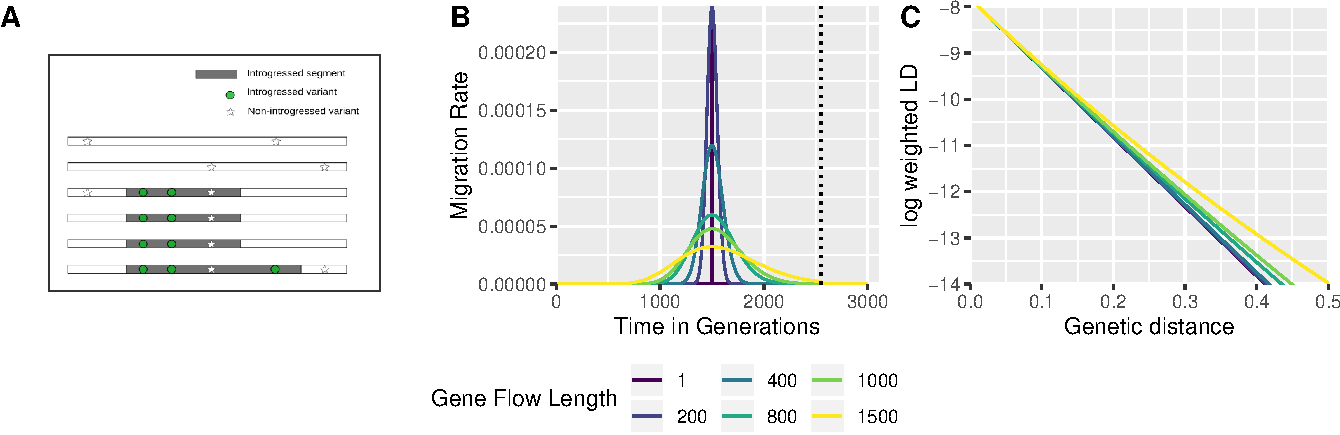
\includegraphics{Admixture_Time_Inference_Paper_Draft_files/figure-latex/fig1-1.pdf}
\caption{\label{fig:fig1} A) Neandertal introgression into non-Africans with a multitude of potential admixture durations. B) The time and duration of admixture results in different length distributions of introgressed chromosomal segments (grey) containing  Neandertal variants (green circles)  in high LD to each other
compared to the background . The ALD approach estimates linkage
between the introgressed variants (green circles), wheres the haplotype approach tries
to estimate the segment directly (grey area). C) Migration rate per generation
modeled using a Gamma distribution for different admixture durations,
dotted line indicates maximum time of gene flow. D) The expected LD
decay under the extended pulse model.}
\end{figure}

\section{Methods}\label{methods}
In this section, we present formal definitions of the admixture models used. 
We conducted simulations to assess the effect of continuous
admixture compared to a pulse under ideal circumstances. 
We also evaluated the impact of different recombination and demographic scenarios and the effect of different analysis parameters for estimates under an instantaneous pulse model.
After assessing these effects we evaluated the possible
parameter range for using the extended pulse model on ALD data,
enabling to obtain a duration of continuous admixture. We use both admixture models on real data. We fitted several admixture scenarios with different durations to ALD data from the 1000 Genomes Project \citep{the_1000_genomes_project_consortium_global_2015} with 3 high coverage Neandertals \citep{prufer_complete_2013,prufer_high-coverage_2017,mafessoni_high_coverage_2020}.

\subsection{Admixture Models}\label{admixture models}

First we need to describe the admixture models used.
Here, we want to define the admixture model in terms of its segment-length distribution $l$ for a random variable $T$ giving the admixture time $t_{admix}$ over the time $t$. 


\begin{equation}
\label{eq:standard_likelihood_definintion}
    P(L=l)=\int_{0}^{\infty} P(T=t) P(L=l | T=t) \ dt
\end{equation}

\subsubsection{The Simple Pulse Model}\label{The Simple Pulse Model}

In the simple pulse model the probability of admixture over time $t$ is given by:

\begin{equation}
\label{eq:RV_simple_pulse}
  P(T)=\left\{
  \begin{array}{@{}ll@{}}
    1, & \text{if}\ T=t_{admix} \\
    0, & \text{otherwise}
  \end{array}\right.
\end{equation} 

Therefore,

\begin{equation}
\begin{split}
\label{eq:Likelihood_function_simple_pulse}
    P(L=l) &=  1  P(L=l | T=t) \\
    &= 1 te^{-tl}
\end{split}
\end{equation}

The expected segment length under a simple pulse model is given by,

\begin{equation}
\label{eq:Expected_l_simple_pulse}
    \mathbb{E}[l]=\frac{1}{t}
\end{equation}

Note that this definition of the segment length distribution is independent from the migration rate $m$ at $t_{admix}$. Hence, the model does not consider the (higher) probability of admixture segments recombining with each other when the migration rate is high. This can be done following Gravel et al. 2012 \citep{gravel_population_2012}. For Neandertal admixture where $m$, the admixture fraction, is typically low, the exponential assumption is satisfied \citep{liang_lengths_2014}.

\subsubsection{The Extended Pulse Model}\label{The Extended Pulse Model}

The extended pulse model as a generalization of the simple pulse model describes multi-generation admixture, where the random variable $T$ follows a continuous mixture distribution $\mathcal{D}_{T}$ instead of just being one discrete value. Specifically that it follows a Gamma distribution with parameters $\Gamma(k,\frac{t_m}{k})$, hence

\begin{equation}
\label{eq:RV_extended_pulse}
  P(T)=\left\{
  \begin{array}{@{}ll@{}}
    \Gamma(k,\frac{t_m}{k}), & \text{if}\ T=t_{admix}\ \text{and}\ k\ \geq 1\\
    0, & \text{otherwise}
  \end{array}\right.
\end{equation} 

with,

\begin{equation}
\begin{split}
\label{eq:RV_extended_pulse_properties}
\mathbb{E}[t]&=t_{m} \\
Var[t]&=\frac{t_{m}^2}{k} = \bigg(\frac{t_d}{4} \bigg)^2  \\
\Gamma(k,\frac{t_m}{k})&= \frac{1}{\Gamma(k)(\frac{t_m}{k})^k}t^{k-1}e^{-t\frac{k}{t_m}}
\end{split}
\end{equation}

Where $t_{m}$ is the mean time of admixture and $Var[t]$ is defined as $(\frac{t_d}{4})^2$ with $t_{d}$ giving the admixture duration.
To get the likelihood function for the segment length distribution $P(L)$ under a multi-generation continuous extended pulse we have to solve the following integral:

\begin{equation}
\label{eq:Likelihood_function_extended_pulse_1}
    P(L=l) = \int_{0}^{\infty} \frac{1}{\Gamma(k)(\frac{t_m}{k})^k}t^{k-1}e^{-t\frac{k}{t_m}}\ t\ e^{-tl} \ dt 
\end{equation}

we can factor out all term not depending on $t$:

\begin{equation}
\label{eq:Likelihood_function_extended_pulse_2}
    P(L=l) = \frac{1}{\Gamma(k)(\frac{t_m}{k})^k}\ \int_{0}^{\infty}\ t^{k-1}e^{-t\frac{k}{t_m}}\ t\ e^{-tl} \ dt 
\end{equation}

we can re-write the integral into the  form of the known integral $\int_{0}^{\infty}\ x^n e^{-\alpha x} \ dx= \frac{\Gamma{n+1}}{\alpha^{n+1}}$

\begin{equation}
\begin{split}
\label{eq:Likelihood_function_extended_pulse_3}
    P(L=l) &= \frac{1}{\Gamma(k)(\frac{t_m}{k})^k}\ \int_{0}^{\infty}\ t^{k}e^{-(l+\frac{k}{t_m})t} \ dt \\ 
    P(L=l) &= \frac{1}{\Gamma(k)(\frac{t_m}{k})^k}\ \frac{\Gamma(k+1)}{l+\frac{k}{t_m})^{k+1}} 
\end{split}
\end{equation}

since $\frac{\Gamma(k+1)}{\Gamma(k)} =k$ we can re-write the likelihood to:

\begin{equation}
\begin{split}
\label{eq:Likelihood_function_extended_pulse_final}
    P(L=l) &= \frac{k}{(\frac{t_m}{k})^k \ (l+\frac{k}{t_m})^{k+1}} \\
    &= \frac{k(\frac{k}{t_m})^k} {(l+\frac{k}{t_{m}})^{k+1}}  \\
    &= \frac{k^{k+1}} { t_{m}^k \ (l+\frac{k}{t_{m}})^{k+1}}  \\
    P(L=l) &= t_{m} \ \Bigg( \frac{k}{t_{m}(l+\frac{k}{t_{m}})}\Bigg)^{k+1}
\end{split}
\end{equation}

The result of equation \ref{eq:Likelihood_function_extended_pulse_final} is a density function known as $Lomax$ or $Pareto-II$-distribution . Hence, we can define the likelihood function for a Gamma distributed extended admixture pulse as being Lomax distributed with parameters $L(k+1,\frac{k}{t_{m}})$, where $k$ can be interpreted as a measure of the duration of the interbreeding.

The expected segment length distribution for the mean time of admixture under the extended pulse model is:

\begin{equation}
\label{eq:Expected_l_extended_pulse}
\mathbb{E}[l] = \frac{1}{t_{m}}
\end{equation}

So the expected segment length distribution for the mean time of admixture between the simple and extended pulse is equal (Eq. \ref{eq:Expected_l_simple_pulse} and  \ref{eq:Expected_l_extended_pulse}). Moreover, as $k$ approaches infinity, we recover the (nested) simple pulse model.

\subsection{Simulations}\label{simulations}

We used the msprime coalescent simulator
\citep{kelleher_efficient_2016} for simulations with sample sizes
chosen to reflect presently available data. For ALD simulations we simulate 176 diploid
African individuals and 170 diploid non-Africans, corresponding to the
number of Yoruba (YRI) and Central Europeans from Utah (CEU)
sequences in the 1000 Genomes project data \citep{the_1000_genomes_project_consortium_global_2015}. Since three
high coverage Neandertal sequences are available \citep{prufer_complete_2013,prufer_high-coverage_2017,mafessoni_high_coverage_2020} we choose to
simulate three diploid genomes. For each individual we simulated 20
chromosomes with a length of 150 Mb each. The mutation rate was set for
all simulations to \(2*10^{-8}\) per base per generation. The
recombination rate was set to \(1*10^{-8}\) per base pair per generation
unless specified otherwise. The demographic parameters are based on
previous studies dating Neandertal admixture
\citep{sankararaman_date_2012,fu_genome_2014,moorjani_genetic_2016}. In
the ``simple'' demographic model (S \ref{fig:figS1} A), the effective
population size is assumed constant at \textit{Ne}=10000 for all populations, the
split time between modern humans and Neandertals is 10000 generations
ago and the split between Africans and non-Africans is 2550
generations ago. The migration rate from Neandertals into non-Africans
was set to zero before the split from Africans, to ensure no Neandertal
ancestry in Africans. Each simulation was repeated 100 times. 


\subsubsection{Simulating admixture}\label{Simulating the expanded pulse}

For our coalescent simulations we used the extended pulse model with $t_m$ as the mean admixture time and $t_d$ as its duration. If $t_d$ is set to 1 (corresponding to a value of k=2250000 since, $k=\frac{t_m^2}{(t_d/4)^2}$) gives the simple pulse model. To obtain the migration rate over time $t$ we simply scaled the Gamma density by the total migration rate from Neandertals to modern humans (here 0.03). 

\subsubsection{Recombination map}\label{recombination map}

Uncertainties in the recombination map were previously shown to bias
admixture time estimates \citep{sankararaman_date_2012,sankararaman_combined_2016,fu_genome_2014}. To investigate the effect of more realistic
recombination rate variation, we simulated samples using a recombination map. For ALD simulations we
either used the African-American-Map \citep{hinch_landscape_2011} or
the HapMap phase 3 \citep{HapMapConsortium_second_2007} for simulations
under a variable recombination rate. For simplicity, we used the same
recombination map (150 Mb of chromosome 1, excluding the first 10 Mb)
for all simulated chromosomes. The mean recombination rate was
calculated from the 150 Mb map (\(1.017 \, \frac{cM}{Mb}\) AAMap and
\(0.992 \, \frac{cM}{Mb}\) HapMap). To examine the effect of uncertainties in the
genetic map we either: used the mean recombination rate from the
respective map to calculate the genetic distance from the physical
distance for each SNP (assuming recombination to be constant), used the other map to assign distances
(e.g.~AAMap used for the msprime simulation and HapMap used to assign
genetic distances, emulating uncertainties in the recombination map) or used the same map for simulation and assigning
genetic distances (population specific map). 

\subsubsection{Complex demography}\label{inferred demography}

Demography such as population size changes are known to influence LD
patterns \citep{gravel_population_2012,liang_lengths_2014}. To test the impact of
demographic history on admixture time estimates, we contsrast our standart model with
realistic and complex demographic histories. This includes substructure in the ancestral human population and additional gene flow between Africans and non-Africans after the Neandertal admixture (S \ref{fig:figS1} B). The 
effective population
sizes are based on estimates from Neandertal and present-day human
genomes. MSMC estimates from YRI as representatives for Africans and CEU
for non-Africans from Schiffles \& Durbin 2014
\citep{schiffels_inferring_2014} were used together with PSMC
\citep{li_inference_2011} inferred demographic model for Neandertals
based on the Vindija33.19 high-coverage genome
\citep{mafessoni_high_coverage_2020}. In order to use the effective
population size estimates at a given time point for modern humans from
Schiffels \& Durbin 2014 for our simulations, we
first transformed the time points given in years back to generations by
using 30 years for one generation, as assumed in Schiffels \& Durbin.
Second, since the original estimates are based on a different mutation
rates (\(1.25*10^{-8} \frac{bp}{gen}\)), we corrected all estimates for
the mutation rate used in the simulations
(\(2*10^{-8} \frac{bp}{gen}\)). The split times between Neandertals and
modern humans was kept the
same as in the simple demographic simulations (10000 generations ago) (S. \ref{fig:figS1} A). In the complex model, we simulated an earlier initial split between populations in Africa 3550 generations ago. With substructure starting from 3200 till the final split at 2550 generations ago with a per generation migration rate between the two subpopulations of 0.001. The population size of the ancestor of Neandertals and
humans before the split was set to 18296 (taken from the MSMC results). To simulate branch shortening
caused by the extinction of Neandertals, Neandertals were sampled 750
generations before the Africans and non-Africans. We simulated an additional admixture event between African and non-African populations with a total migration rate of 0.01 starting from 200 till 50 generations ago.

\subsection{Admixture time estimates}\label{admixture time estimates}

For our estimates we do not infer the segments length directly, rather using the decay of admixture-induced LD. This is straight forward, since the formulas given in \ref{eq:Likelihood_function_simple_pulse} and \ref{eq:Likelihood_function_extended_pulse_final} can be easily adapted by considering $P(D=d)$ at a given distance $d$ in Morgan instead of the length $l$. Therefore, we calculated the LD between Neandertal informative sides a given distance $d$ apart from each other.

\subsubsection{Ascertainment scheme}\label{asceteinment scheme}

For the ALD method, SNPs need to be ascertained to enrich for
Neandertal informative sites in the test population to remove noise and
amplify the ALD signal \citep{sankararaman_date_2012}. 
We evaluated the impact of the ascertainment scheme by contrasting two distinct schemes \citep{sankararaman_date_2012,fu_genome_2014}. The lower-enrichment
ascertainment scheme (LES) filters for SNPs fixed for the ancestral state in
Africans and polymorphic in Neandertals. The higher-enrichment
ascertainment scheme (HES) restricts the analysis on SNPs fixed for the
ancestral state in Africans, polymorphic in Neandertals and polymorphic
in non-Africans.

\subsubsection{ALD calculation and curve fitting}\label{ALD calculation and curve fitting}

The pairwise weighted LD between the ascertained SNPs a certain genetic
distance \(d\) apart was calculated using ALDER
\citep{loh_inferring_2013}. A minimal genetic distance \(d_0\) between
SNPs was set either to 0.02 cM and 0.05 cM. This minimal distance cutoff
removes extremely short-range LD, which might be due to incomplete lineage sorting (ILS). As a result of using cutoffs we used the complement cumulative distribution of the likelihood functions given in \ref{eq:Likelihood_function_simple_pulse} and \ref{eq:Likelihood_function_extended_pulse_final} describing $P(D \geq d_0)$ (Eq. \ref{eq:simple_pulse_ccdf} and \ref{eq:extended_pulse_ccdf}). Here \emph{A} is the
intercept, $t_m$ the mean time since the admixture event in generations,
\emph{d} the genetic distance in cM and \emph{c} is a constant modeling
background LD. The simple pulse model was fitted following Moorjani et al 2016
\citep{moorjani_genetic_2016} (Eq. \ref{eq:simple_pulse_ccdf}). The extended pulse model is
modeled using the Lomax ccdf (Eq. \ref{eq:extended_pulse_ccdf}).  We fitted the distribution to the data using a non-linear least-square optimization algorithm
implemented in R \citep{R_Core_Team_2019}.




\begin{equation}
\label{eq:simple_pulse_ccdf}
ALD \sim\ A\,e^{-t_m \:d}+c
\end{equation}

\begin{equation}
\label{eq:extended_pulse_ccdf}
ALD \sim\ A\,\left( \frac{1}{1 + \frac{k}{tm} \:d}\right) ^k+c
\end{equation}


\subsection{Modeling parameter effect sizes}\label{modeling prameter effect sizes}

To model and compare parameter effect sizes we simulated 100
replicates for each combination of
parameters: ascertainment scheme ($A_i$ = LES/HES), minimal genetic distance
($M_i$ = \(d_{0}=0.02\,cM\)/\(d_{0}=0.05\,cM\)), demography ($D_i$ = simple/complex),
recombination rate ($R_i$ = constant/variable), admixture model
($G_i$ = pulse/continuous). Results of simulations where the nls-optimization to
fit the ALD decay curve did not converge were removed (10 out of 3200).
We used a Generalized Linear Model (GLM)  to estimate the effect
size of the different parameters (Eq.
\ref{eq:8}). The difference between the estimated
admixture time and the true admixture time, the error in the estimate,
was standardized using the true time as the mean. The standardized error in this model is the response to the parameters as model
predictors. We choose the Normal distribution as the likelihood function being the maximum entropy distribution in our case. The mean of the Normal distribution is then described by a fixed effect size model of the predictors (factors) coded as indicator variables. We obtained the posterior probability using a Hamiltonian Monte Carlo MCMC algorithm, as implemented in STAN \citep{carpenter_stan_2017} using an R interface \citep{stan_development_team_rstan_2018,mcelreath_statistical_2020}. The Markov chains converged to the target distribution (Rhat = 1) and efficiently sampled from the posterior (S Table \ref{tab:tableS1}).  

\begin{equation}\label{eq:8}
\begin{split}
E_i &\sim Normal(\mu_i,\sigma) \\
\mu_i &= \alpha + \beta_aA_i + \beta_mM_i + \beta_dD_i + \beta_rR_i + \beta_gG_i \\
\alpha &\sim Normal(0,2) \\
\beta_a,\beta_m,\beta_d,\beta_r,\beta_g &\sim Normal(0,2) \\
\sigma &\sim Exponential(1)
\end{split}
\end{equation}

\subsection{Estimating admixture time from real data}\label{Estimating admixture time from real data}

We applied the extended pulse model on real data to see if we can reject any admixture durations (including a one generation pulse), by comparing the model fit to the data for different duration parameters.
We used the 1000 Genomes phase 3 data together with the Altai, Vindija and Chagyrskaya high coverage Neandertals.  We filtered for all unrelated individuals from the YRI as representatives of unadmixed Africans and all CEU as admixed Europeans. We only considered biallelic sites. The sites were polarized relative to the Chimpanzee base (panTro4). We used the CEU specific fine-scale recombination map \citep{spence_inference_2019} to convert the physical distance between sites into genetic distance. 

\section{Results}\label{results}

\subsection{Introduction to result}\label{introduction to result}

We used coalescent simulations of Neandertal admixture into non-African humans to investigate multi-generation continuous admixture, using a Gamma distribution describing the per generation migration rate (the extended pulse model). Focusing on the ALD approach, we used the ALDER program to infer the decay of LD between ascertained sites informative for Neandertal introgression in non-Africans. The ascertained ALD was fitted with an exponential distribution assuming a one-generation admixture pulse (the simple pulse model).  We simulated this scenario using different conditions of recombination and demography as well as deploying different ascertainment schemes and LD cutoffs. A Generalized Linear Model (GLM) was used to compare all these factors with the effect of an extended pulse on the one-generation assumption. The Lomax distribution describing the ALD under an extended admixture pulse was deployed for fitting the data to obtain the duration of admixture. We test this new fitting with the most inferential factors from the previous analysis on simulated and real data using the ALD.


\subsection{The effect of continuous admixture on the admixture time estimates}\label{the effect of continuous admixture on the admixture time estimates}


To assess the effect of estimating admixture time assuming a one-generation pulse when the real gene flow is actually continuous over multiple generations,
we compared the mean average deviation from the true mean time of admixture for simulations under a simple pulse with the one under an extended pulse with the same mean time.
The total amount of gene flow \(m\) from Neandertals into non-Africans
in the two models is equal. 
The shape and scale parameter of the Gamma distribution modeling the migration rate are chosen such
that the resulting weighted LD decay curves as functions of genetic
distance share the same mean for both admixture models. We used the LES ascertainment scheme and a minimal distance between SNPs of 0.05 cM. 

First, we evaluate the effect of the admixture time on the accuracy of both a single pulse and an extended pulse model. The mean admixture times ranges
from 250 generations ago to 2000 generations ago.  The duration
of interbreeding under the extended pulse model is 50\% of the mean time (if the
mean time is 250 generations ago gene flow ranges from 325 to 175
generations ago). Assuming only a one generation pulse to estimate the
mean time, revealed only minor deviations between the two scenarios and
the true admixture time of 3\% to 6\% for the simple pulse and 0\% to 5\% for
the extended pulse (Figure \ref{fig:fig2} A).



To
further investigate the effect of simple and extended pulse gene flow on the
admixture time estimates, we compared different durations of 
admixture with a fixed mean time of admixture of 1500
generations ago, displayed in Figure \ref{fig:fig2} B. Estimates between
simple and extended admixture pulse start to deviate for 800 generations of
continuous admixture, with increasingly lower estimates for simulations
under continuous admixture compared to simulations under a one-generation pulse scenario per increase of admixture duration.

This bias is likely caused
by the differences in LD between sites entered in the tails of the gamma
distribution. LD between sites arising from early admixture events,
simulated by the right tail of the gamma distribution, is not detected
anymore, while LD between sites from late admixture is still present,
biasing the estimate towards younger dates. 

However, deviations in
estimates between the two scenarios of \textasciitilde{}120 generations
in the most extreme case are moderate compared to the mean admixture
time of 1500 generations.

In summary, the differences in mean time estimates between the simple and extended pulse admixture assuming a one-generation pulse to estimate the time are moderate, even for very long continuous admixture scenarios. This makes point estimates for mean admixture time compatible with long continuous admixture.


\begin{figure}
\centering
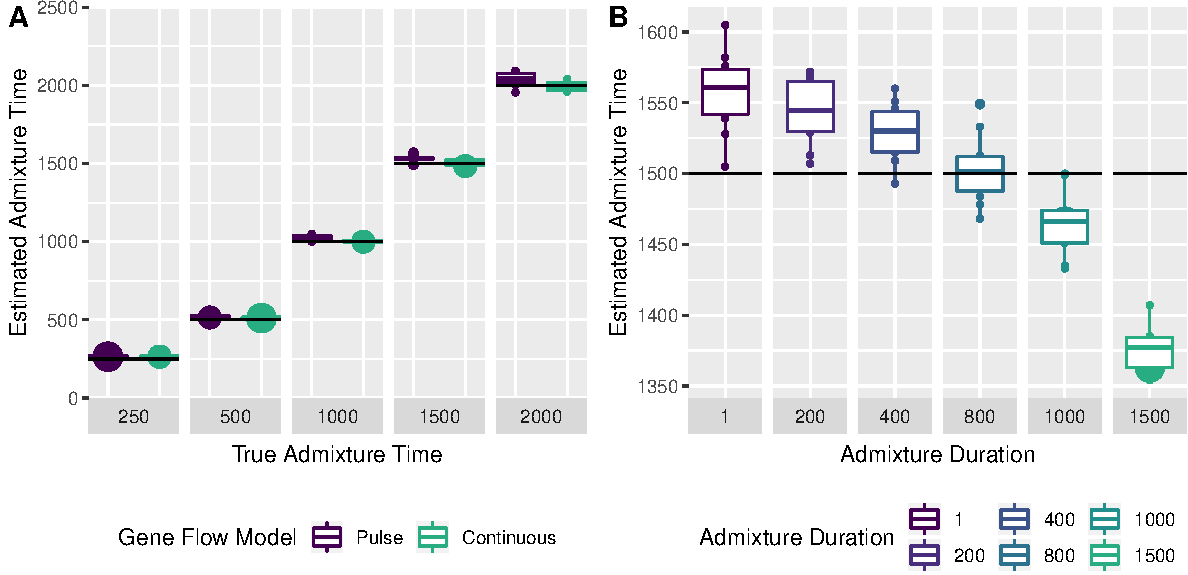
\includegraphics{Admixture_Time_Inference_Paper_Draft_files/figure-latex/fig2-1.pdf}
\caption{\label{fig:fig2} A) Comparison of mean admixture time estimates
between pulse and continuous gene flow for different admixture times.
The length of continuous gene flow corresponds to 50\% of the mean
admixture time, black line indicates true mean admixture time. B)
Comparison of mean admixture time estimates for simulations with a mean
time of admixture of 1500 generations ago, at a varying length of gene
flow. Boxplot created from 100 simulation replicates, respectively.}
\end{figure}
\subsection{Comparing effect sizes}\label{comparing effect sizes}

Having shown that the duration of continuous admixture under ideal
circumstances only marginally influences admixture time
estimates, we want to compare its effect in more realistic simulation scenarios. Two common assumptions, namely knowing the recombination pattern and knowing the demographic history, were implicitly used in the previous simulations.
Previous studies reported that violations of these assumptions can have an effect on the admixture time estimates.
Hence, we used the African-American genetic map and a more complex demography with substructure in the ancestral human population and additional gene flow between Africans and non-Africans after the Neadertal admixture ended (S. \ref{fig:figS1} B), for simulations under more realistic parameters. The genetic distance was assigned using the average recombination rate of the African-American genetic map (assuming a constant recombination rate).
Furthermore, we altered the used scheme for ascertainment of SNPs for admixture informative sites. We compared the LES where only
positions in the admixed population are considered where both source
populations are diverged from each other, to an even stricter scheme. The Higher-Enrichment Scheme (HES) requiring additional
to the LES non-Africans to be polymorphic at a SNP. Additionally, we altered the minimal distance between pairs of SNPs for which the LD is calculated from 0.05 cM to 0.02 cM.



We simulated every combination of these parameter sets resulting in 32
different sets with 100 replications each (S. \ref{fig:figS2}).
A GLM was applied to estimate effect sizes of the four predictors being
ascertainment scheme, minimal distance, demography and recombination on
the bias of admixture estimates (Supplement Table \ref{tab:tableS1}).
Figure \ref{fig:fig3} shows the comparison of the standardized
difference between true and estimated time between the previously used
model (ascertainment = LES, \(d_{0} = 0.05 cM\), demography = simple and
recombination = constant) further referred to as the standard model and
a model with one of the four parameter changed, respectively. The
previously observed overestimation of the standard model was estimated
to be 0.12 (0.08 - 0.16 95 \% CI) standard deviation from the true
admixture time.

Every parameter change, except using \(d_{0} = 0.02 cM\), results in lower estimates compared to the
standard model, with the biggest difference between a constant and a
varying recombination (-1.76 - -1.7 95 \% CI). The
underestimation caused by the extended admixture pulse (-0.34 -
-0.28 95 \% CI) is in the range of biases arising from the ascertainment scheme (-0.35 -
-0.29 95 \% CI) and only slightly more then caused by a more complex demography (-0.25 -
-0.19 95 \% CI). Most accurate estimates are achieved using the LES
ascertainment scheme in combination with a minimal distance of 0.05 cM.
Additionally, the bias introduced by the demography seems to depend on
the used ascertainment scheme, since only under the HES a difference
between the simple and complex demography is evident (S.
\ref{fig:figS2}).

Overall the bias introduced by the ascertainment, minimal distance
cutoff, demography and admixture model are  around +/-0.25 standard deviations or less. The major uncertainties in the admixture time
estimate arise from assuming a constant recombination rate. The
admixture time estimates for a simple or extended admixture pulse are similarly effected by the other modeling parameters.

\begin{figure}
\centering
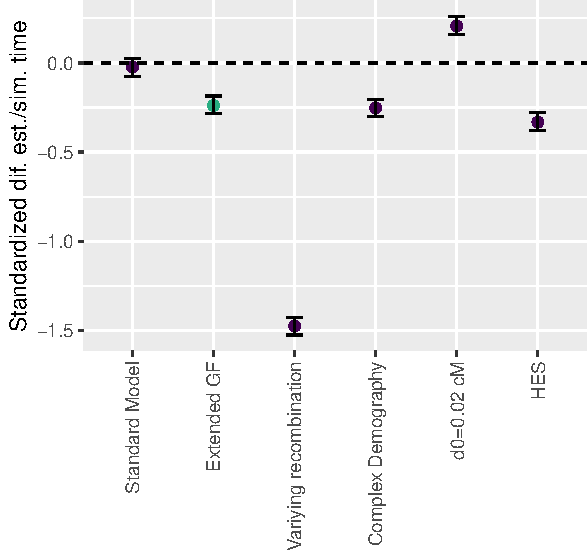
\includegraphics{Admixture_Time_Inference_Paper_Draft_files/figure-latex/fig3-1.pdf}
\caption{\label{fig:fig3} Effect size estimates for each parameter on the standardized difference between true and estimated admixture time. Dotted horizontal line indicates unbiased admixture estimates.}
\end{figure}

\subsection{Estimating the Lomax-parameters under different conditions}\label{estimating the Lomax-parameters under different conditions}

Building on the previous
result we want to find out the conditions to retrieve the Lomax
parameters i.e.~the duration of the admixture. We simulated an admixture
scenario under a simple demography with varying durations of an extended
admixture pulse and sampled the population at different time points since the
end of the interbreeding. Doing so allows us to examine how close one has to
sample form the end of a continuous admixture to still accurately
estimate its duration. Since the recombination map was shown to be highly
influential, we tested the duration estimates under a constant and variable
recombination using the HapMap genetic map. Here, we correct the
genetic distance by: assuming a constant rate, using the AAMap (uncertainty in the recombination map) or the
HapMap itself (having a  population specific recombination map). We used the LES ascertainment scheme in combination with
a minimal distance of 0.05 cM.  Figure \ref{fig:fig4} A and C show the mean
time estimates received from the Lomax fit. For simulations under a
constant recombination the mean time can be estimated confidently for different durations and different sampling times after the end of the admixture event. Estimates for simulation under a recombination map only
assuming a constant rate when calculating the LD results in high uncertainty and overestimation. This is different for estimates under an Exponential distribution (S.  \ref{fig:figS3}). Using the AAMap yields
results closer to the true value and less biased, however only
using the exact same genetic map gives unbiased results. Figure
\ref{fig:fig4} B and D shows the corresponding admixture duration estimates by the
Lomax fit. Accurate estimates can be obtained throughout the different
admixture durations under a constant recombination rate, when sampled
recently from the end of the continuous admixture. Sampling further away from the end of the admixture results in less accurate estimates.  All simulations using a recombination map show a much higher
variance in the estimates. Especially for admixture durations longer then
800 generations or sampled later then 50 generations away from the end
of the admixture, the estimates are not reliably. If no precise genetic map
is used to infer the genetic distance between SNPs, no accurate
duration estimates can be obtained. Even for estimates using the population specific map, the variation is considerable for admixture durations longer then 800 generations or sampled later then 200 generations after the end of the gene flow.

Under a realistic scenario with a varying recombination
rate, the duration can only be accurately estimated with a highly
precise map for recent continuous admixture events not longer then 400
generations. With regard to scenarios of Neandertal admixture,
accurately estimating the duration of possible continuous admixture from
present day human genomes even under a constant rate seems
under powered. 


\begin{figure}
\centering
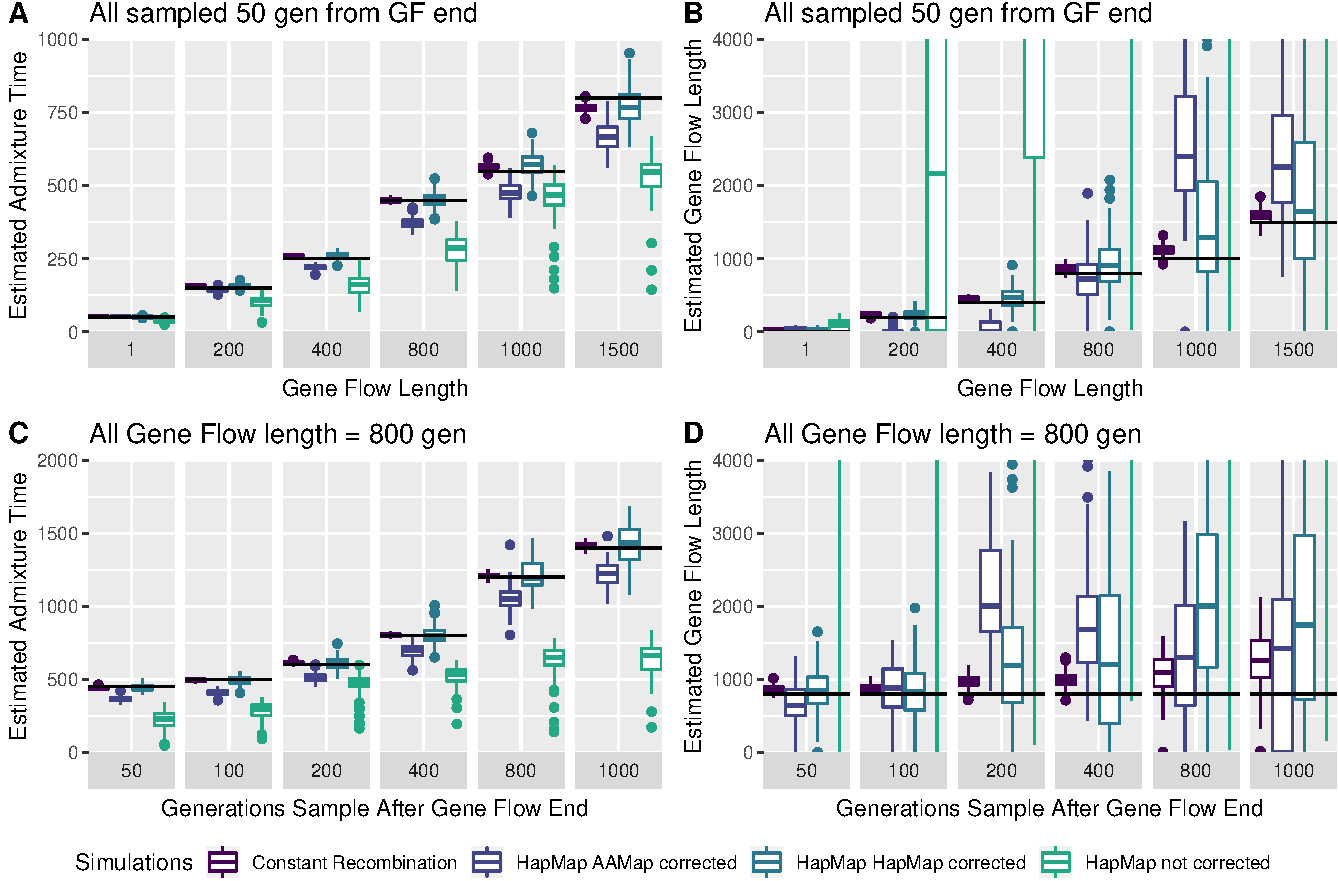
\includegraphics{Admixture_Time_Inference_Paper_Draft_files/figure-latex/fig4-1.pdf}
\caption{\label{fig:fig4} Lomax parameter estimate for different sampling and
admixture duration times using different methods for assigning genetic
length A) Mean time estimates for different gene
flow length all sampled 50 generations after the gene flow ended. B)
Duration estimate of the scenario C) Mean time estimates for different sampling times after the end of 800
generations of gene flow. D) Duration estimate of the scenario}
\end{figure}


We can also demonstrate this using real data.
Figure \ref{fig:fig5} (S. Table \ref{tab:tableS2}) shows multiple admixture duration scenarios ranging from a one generation pulse to 2500 generations of continuous admixture. All scenarios are compatible with the ALD data from 1000 Genome's CEU computed using YRI and the Altai, Vindija and Chagyrskaya high coverage as reference populations and a CEU specific fine-scale genetic map \citep{spence_inference_2019}.



\begin{figure}
\centering
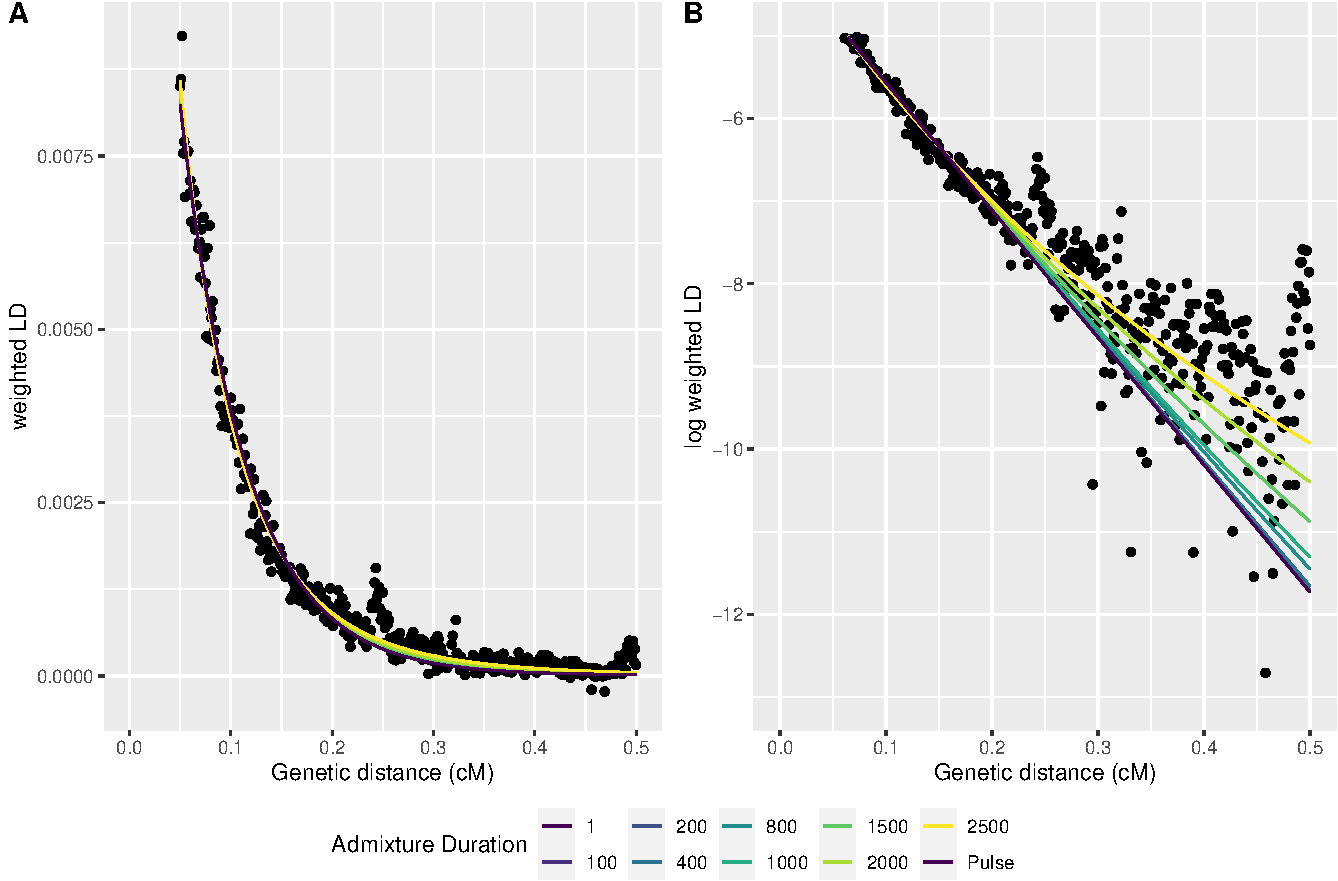
\includegraphics{Admixture_Time_Inference_Paper_Draft_files/figure-latex/fig5-1.pdf}
\caption{\label{fig:fig5} Different admixture duration models ranging
from a one generation pulse to 2500 generations of gene flow for Neandertal interbreeding using all 1k Genome CEU individuals as the admixed population
with all YRI and 3 high coverage Neandertals as reference populations. A) Weighted LD normal scaled B) Weighted LD log scaled.}
\end{figure}

\section{Discussion}\label{discussion}

How, where and when Neandertals and early modern humans interacted remains contentious.  
Archaeological evidence bounds the timing of interactions to times when their range overlapped; from the first out-of-Africa migrations of modern humans around 188 k years ago \citep{stringer_when_2018,hershkovitz_earliest_2018} to the extinction of Neandertals around 37 - 39 kya \citep{higham_timing_2014,zilhao_precise_2017}, leaving a time-span of roughly 140ky in which interbreeding between modern humans outside of Africa and Neandertals might be feasible.

Genetic data has revealed that gene flow between Neandertals and modern humans did occur \citep{green_draft_2010}; and it's mean age is estimated to 47,000–65,000 ya (\citep{sankararaman_date_2012}), under a single pulse model, but later interbreeding has been documented \citep{fu_early_2015}.

Here, we contrasted this pulse model with scenarios involving more long-standing gene flow.  Our model, assumes that migration rates  follow a Gamma distribution, which results in a simple closed-form expression for the introgressed segment lengths or ALD  distributions. 

In our analyses using the extended model, we find that mean admixture time estimates vary little between models. However, we also show that even gene flow lasting thousands of generations may yield data that are practically indistinguishable from a one-generation pulse, and that other modelling and method assumptions have an impact on estimates that are of a similar magnitude or much higher. Particularly assumptions on the recombination rate are highly impactfull, and will lead to sever underestimations of admixture times. Therefore reliable mean time estimates can only be obtained using population specific recombination maps.

The major implication of our result is that interpreting results of genetic dating is difficult.  Estimating the mean time of gene flow and its confidence intervals are not indicative of the actual duration of the interbreeding.  This is of great practical importance as it might be tempting to link the genetic admixture date estimates with biogeographical events \citep{sankararaman_date_2012,lazaridis_genomic_2016,jacobs_multiple_2019,vyas_analyses_2019,douka_age_2019}. For example, the lower bounds on admixture time estimates might be used as dates of Neandertal extinction, and likewise use the earliest dates of gene flow as evidence when the out-of-Africa migration happened \citep{sankararaman_date_2012}. Our results show that both of these interpretations might be misleading. However, using the extended pulse model relaxing the one generation pulse assumptions used for earlier estimates, also indicates that most of the gene flow was around 45,000 to 65,000 years ago, consistent with previous estimates.


While our results show that drawing concrete conclusions from admixture time estimates can be misleading, other avenues for differentiating different gene flow events remain fruitful.
In particular, measures based on population differentiation (e.g \citep{browning_analysis_2018,wall_higher_2013,villanea_multiple_2019}) are very promising to understand the different events that contributed to archaic ancestry in present-day humans. 

The other major avenue are ancient DNA samples from early modern humans that lived around or immediately after gene flow between archaic and modern humans occurred. The \textit{Oase 1} \citep{fu_genome_2014} genome is a prime example, as it directly demonstrates that some gene flow must have occurred in Europe, around 40,000 years ago, concurrently with when \textit{Oase 1} lived. More generally, detailed analyses of ancient genomes from the initial upper paleolithic should provide more accurate mean dates, as they are much closer to the gene flow, and may give better evidence about the duration of the gene flow. The drawback is that some of the gene flow these individuals experience may be private to their population, as has e.g. been suggested for \textit{Oase 1}. Larger numbers of early modern human genomes, as well as methods to accurately infer admixture tracts or ALD in low-coverage data will likely enable this line of research. 


\hypertarget{refs}{}

\bibliography{References/MyLibraryATE}


\pagebreak
\setcounter{figure}{0} \renewcommand{\figurename}{Fig. S}
\renewcommand{\tablename}{Tab. S}

\section{Supplement}\label{supplement}

\begin{figure}
\centering
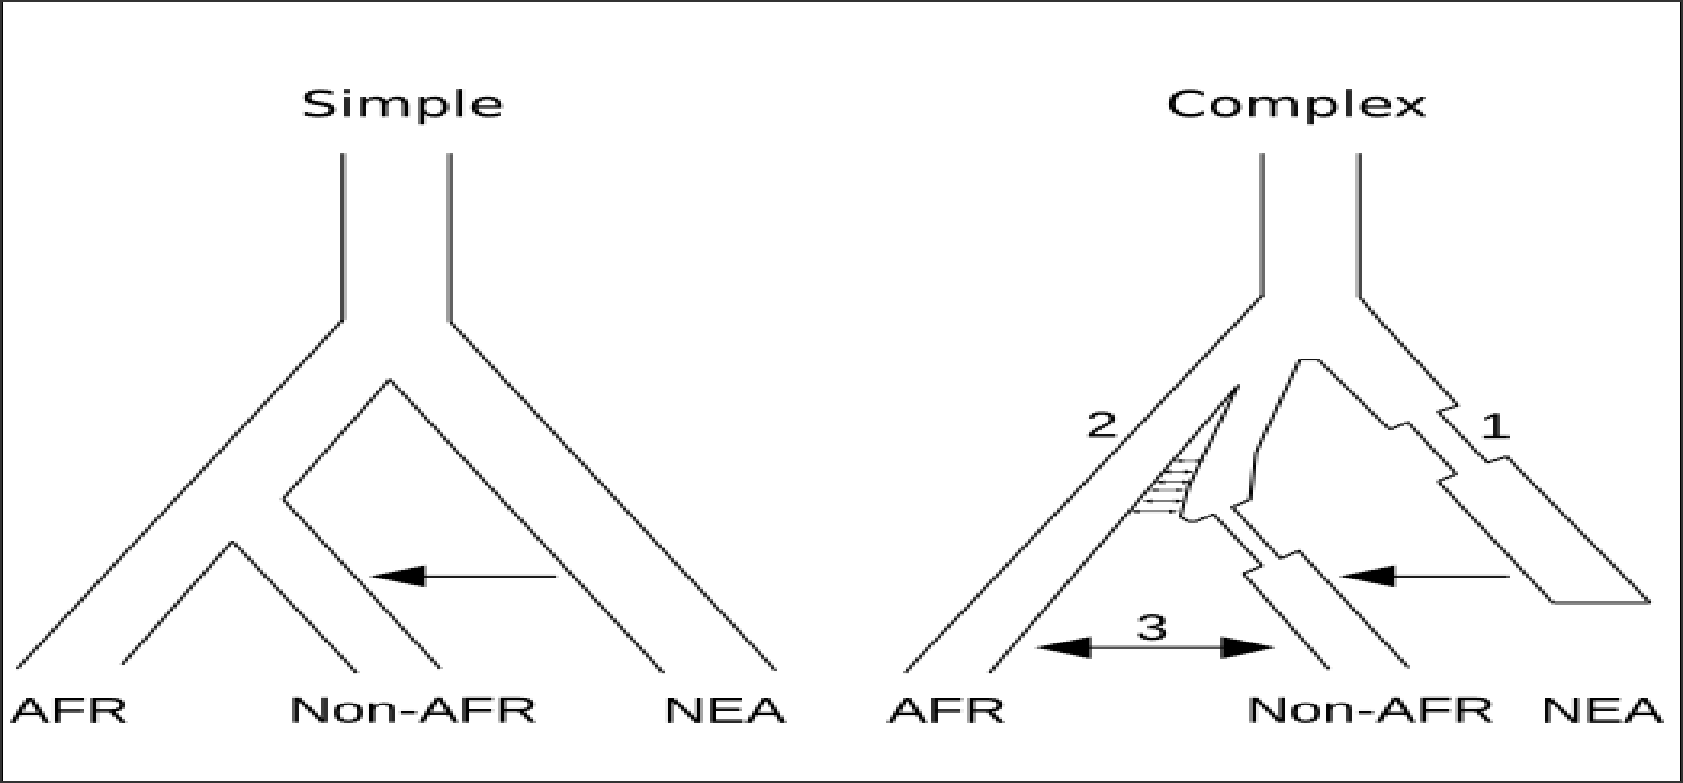
\includegraphics{Admixture_Time_Inference_Paper_Draft_files/figure-latex/figS1-1.pdf}
\caption{\label{fig:figS1} Demographic models of Neandertal admixture with non-Africans used for the simulations. A) Simple demographic model used for ALD simulations with constant population sizes. B) Complex demographic model with substructure in Africa, where after an initial earlier split and isolation the structured population exchange migrants till the final split and additional gene flow between Africans and non-Africans after the Neandertal admixture. The  population sizes after the (final) split are taken fome MSMC/PSMC estimates for the respective populations. C) Demographic model for the direct inference of Neandertal segments in non-Africans taken and modified from Skov et al. 2018. (\citep{skov_detecting_2018})}
\end{figure}

\begin{figure}
\centering
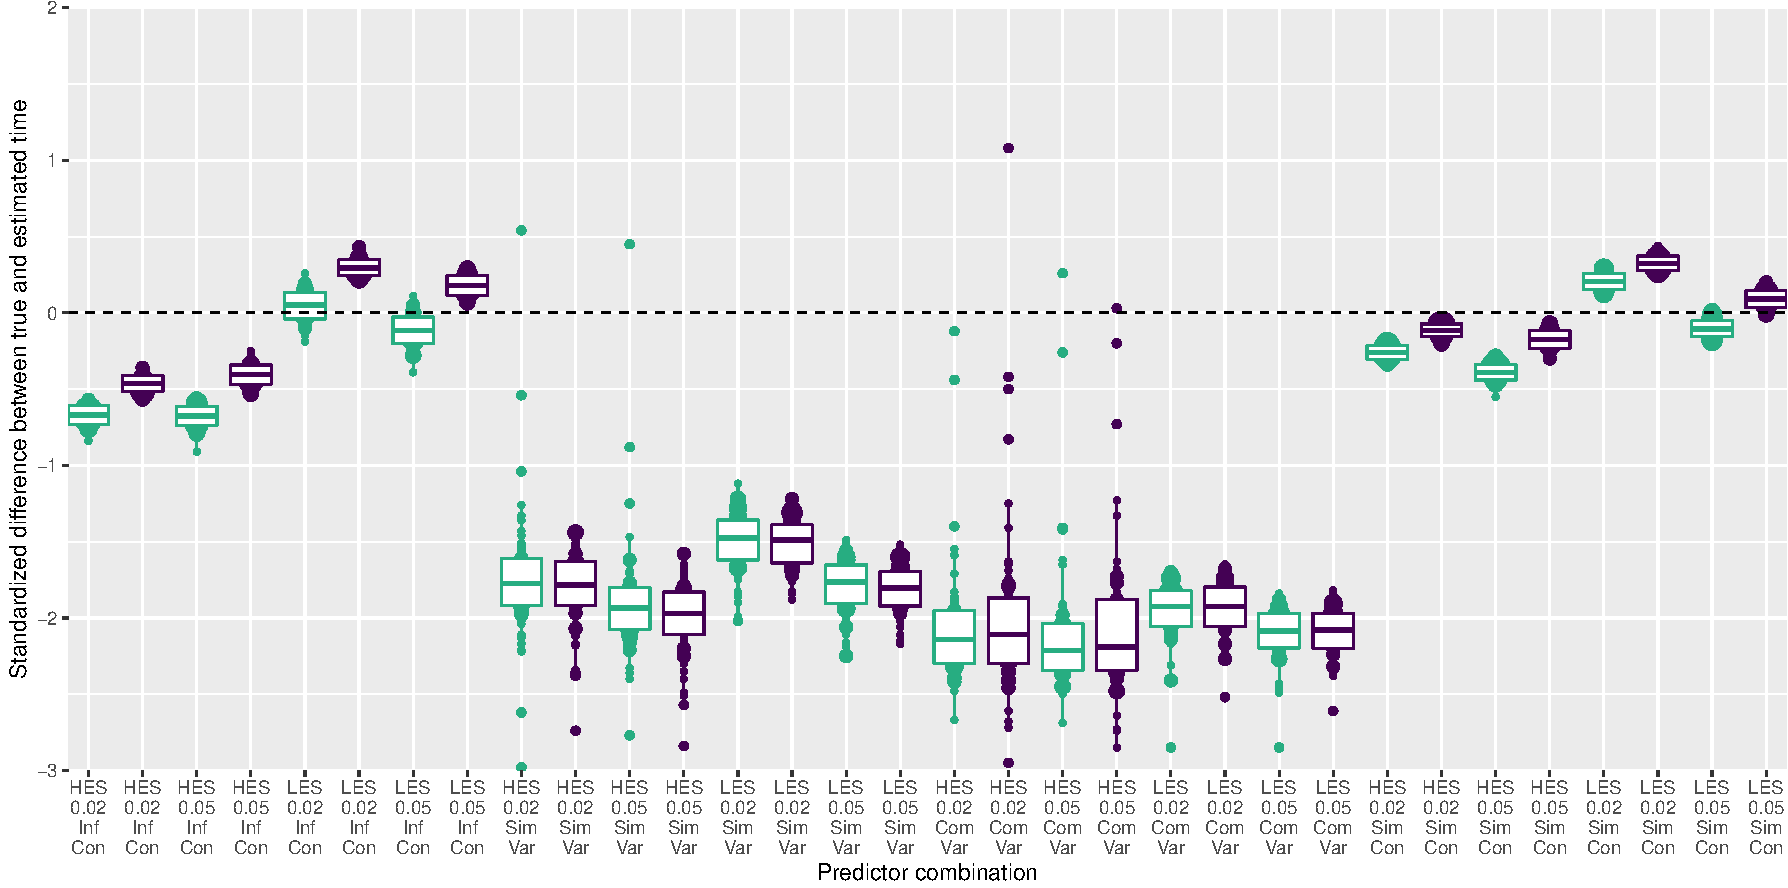
\includegraphics{Admixture_Time_Inference_Paper_Draft_files/figure-latex/figS2-1.pdf}
\caption{\label{fig:figS2} Comparison of the standardized difference between true and estimated admixture time for all combinations of parameters: ascertainment scheme = LES/HES,  $d_{0}$ = 0.02/0.05 cM, demography = simple/complex, recombination = constant/variable and the gene flow model = pulse/continuous, with 100 replicates respectively. Dotted horizontal line indicates no difference between true and estimated time.}
\end{figure}

\begin{table}[H]

\caption{\label{tab:tableS1}\label{tab:tableS1} Mean, standart deviation, 5.5/94.5 compatibility interval of the posterior distribution for every parameter effect on the standardized difference between true and estimated admixture time.}
\centering
\begin{tabular}{l|r|r|r|r|r|r}
\hline
  & mean & sd & 5.5\% & 94.5\% & n\_eff & Rhat\\
\hline
a & 0.12 & 0.02 & 0.08 & 0.16 & 1220.94 & 1\\
\cline{1-7}
bG & -0.31 & 0.02 & -0.34 & -0.28 & 1559.84 & 1\\
\cline{1-7}
bR & -1.73 & 0.02 & -1.76 & -1.70 & 2112.69 & 1\\
\cline{1-7}
bD & -0.22 & 0.02 & -0.25 & -0.19 & 2036.66 & 1\\
\cline{1-7}
bm & 0.13 & 0.02 & 0.10 & 0.17 & 1657.66 & 1\\
\cline{1-7}
bA & -0.32 & 0.02 & -0.35 & -0.29 & 1721.62 & 1\\
\cline{1-7}
sigma & 0.46 & 0.01 & 0.44 & 0.47 & 2239.47 & 1\\
\hline
\end{tabular}
\end{table}

\begin{figure}
\centering
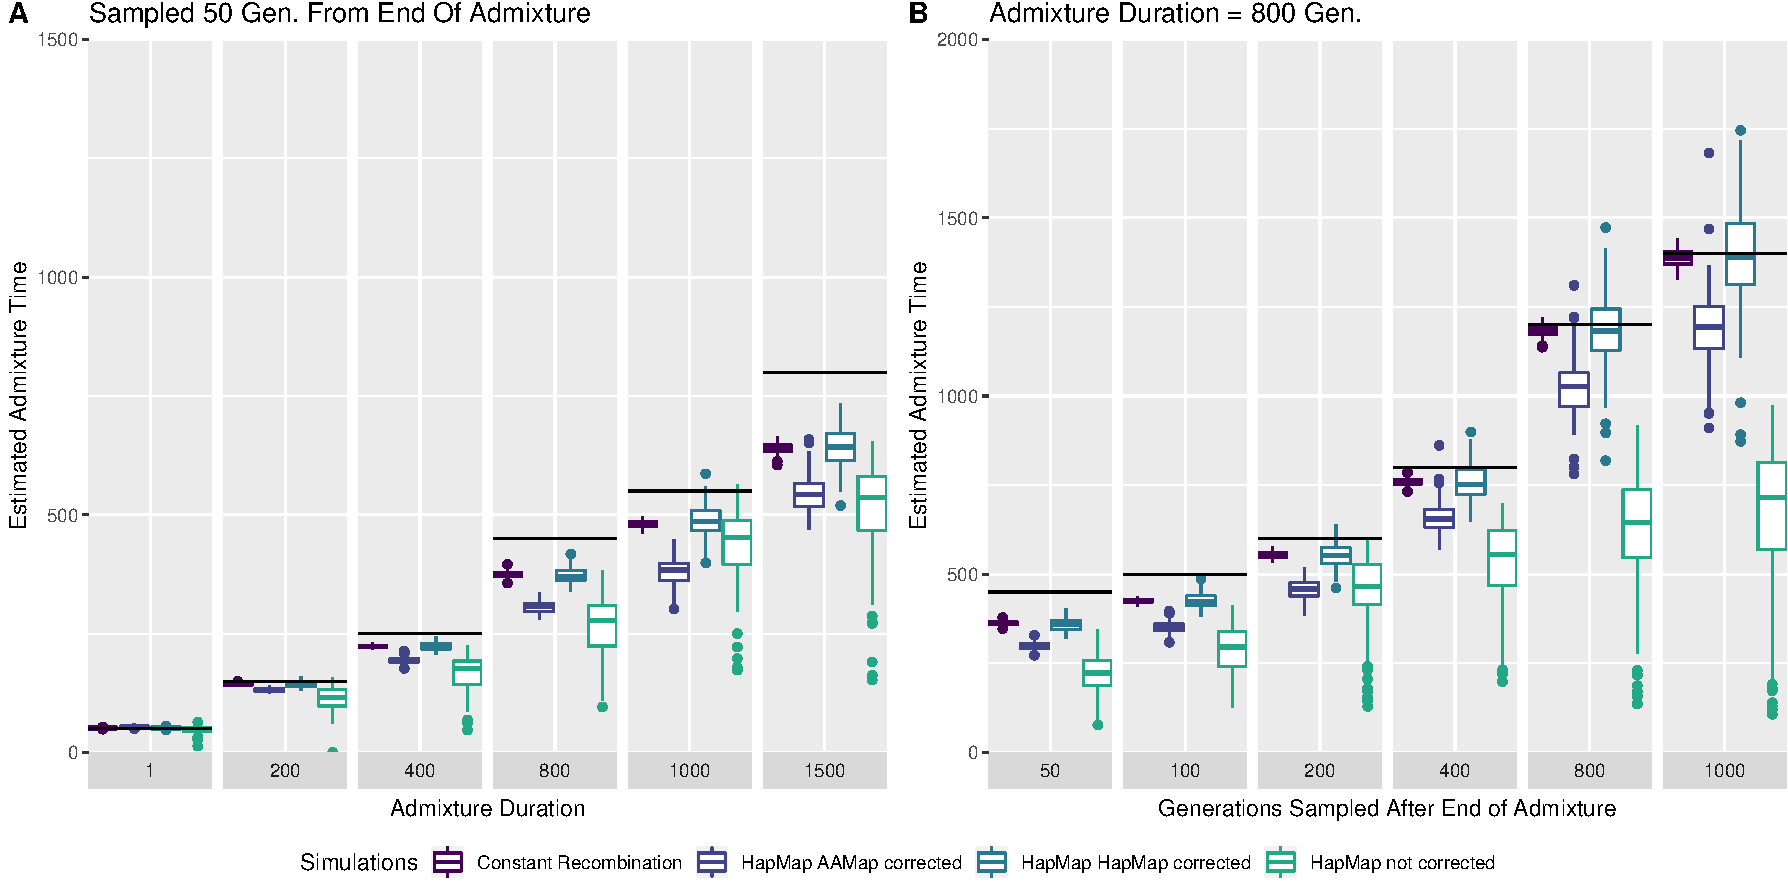
\includegraphics{Admixture_Time_Inference_Paper_Draft_files/figure-latex/figS3-1.pdf}
\caption{\label{fig:figS3} Mean time estimates of the Exponential model A) Mean time estimates for different 
admixture durations all sampled 50 generations after the admixture ended. B) Mean time estimates for different sampling times after the end of 800
generations of continuous admixture.}
\end{figure}

\begin{table}[H]
\caption{\label{tab:tableS2}\label{tab:tableS2} Mean and 2.5/97.5 compatibility interval for every parameter estimated in the model fit}
\centering
\begin{tabular}{l|l|l|l|l}
\hline
Model & Parameter & Estimate & 2.5 \% & 97.5 \%\\
\hline
Exponential & A & 0.0177951442439937 & 0.0177907714786252 & 0.0177995170093623\\
\hline
Exponential & mean time & 1540.51741259424 & 1486.87051449324 & 1598.18041766271\\
\hline
Exponential & c & 1.04922402241663e-05 & 6.11947485562607e-06 & 1.48650055927066e-05\\
\hline
Lomax (td=1) & A & 0.0177951442439937 & 0.0177907714786252 & 0.0177995170093623\\
\hline
Lomax (td=1) & mean time & 1540.54690341371 & 1486.89897832594 & 1598.21101235108\\
\hline
Lomax (td=1) & c & 1.04949518630901e-05 & 6.12218649454983e-06 & 1.48677172316303e-05\\
\hline
Lomax (td=100) & A & 0.0177951442439937 & 0.0177907714786252 & 0.0177995170093623\\
\hline
Lomax (td=100) & mean time & 1541.21552745233 & 1487.54431823588 & 1598.90466361173\\
\hline
Lomax (td=100) & c & 1.04778971116211e-05 & 6.10513174308087e-06 & 1.48506624801614e-05\\
\hline
Lomax (td=200) & A & 0.0177951442439937 & 0.0177907714786252 & 0.0177995170093623\\
\hline
Lomax (td=200) & mean time & 1543.30241011905 & 1489.55852740936 & 1601.0696602451\\
\hline
Lomax (td=200) & c & 1.04341296352963e-05 & 6.06136426675609e-06 & 1.48068950038366e-05\\
\hline
Lomax (td=400) & A & 0.0177951442439937 & 0.0177907714786252 & 0.0177995170093623\\
\hline
Lomax (td=400) & mean time & 1551.70459843938 & 1497.66811836146 & 1609.78635031902\\
\hline
Lomax (td=400) & c & 1.02583870973029e-05 & 5.88562172876263e-06 & 1.46311524658431e-05\\
\hline
Lomax (td=800) & A & 0.0177951442439937 & 0.0177907714786252 & 0.0177995170093623\\
\hline
Lomax (td=800) & mean time & 1586.19945700954 & 1530.96172977427 & 1645.57238365183\\
\hline
Lomax (td=800) & c & 9.54350178205991e-06 & 5.17073641351966e-06 & 1.39162671506002e-05\\
\hline
Lomax (td=1000) & A & 0.0177951442439937 & 0.0177907714786252 & 0.0177995170093623\\
\hline
Lomax (td=1000) & mean time & 1613.04056713235 & 1556.86812647683 & 1673.41818158693\\
\hline
Lomax (td=1000) & c & 8.99447037087496e-06 & 4.62170500233471e-06 & 1.33672357394152e-05\\
\hline
Lomax (td=1500) & A & 0.0177951442439937 & 0.0177907714786252 & 0.0177995170093623\\
\hline
Lomax (td=1500) & mean time & 1713.23411309364 & 1653.57253761458 & 1777.36206551997\\
\hline
Lomax (td=1500) & c & 6.99221511836012e-06 & 2.61944974981987e-06 & 1.13649804869004e-05\\
\hline
Lomax (td=2000) & A & 0.0177951442439937 & 0.0177907714786252 & 0.0177995170093623\\
\hline
Lomax (td=2000) & mean time & 1874.70574615156 & 1809.42109093705 & 1944.87773256239\\
\hline
Lomax (td=2000) & c & 3.90606333903974e-06 & -4.66702029500504e-07 & 8.27882870757999e-06\\
\hline
Lomax (td=2500) & A & 0.0177951442439937 & 0.0177907714786252 & 0.0177995170093623\\
\hline
Lomax (td=2500) & mean time & 2128.77896518946 & 2054.64647743473 & 2208.46114940615\\
\hline
Lomax (td=2500) & c & -6.57497391994452e-07 & -5.0302627605347e-06 & 3.7152679765458e-06\\
\hline
\end{tabular}
\end{table}



\end{document}